\documentclass{article}
\usepackage[utf8]{inputenc}
\usepackage[margin=1in]{geometry}
\usepackage{graphicx}
\usepackage{hyperref}
\hypersetup{
    colorlinks=true,
    linkcolor=blue,
    filecolor=magenta,
    urlcolor=black,
}
\newcommand{\n}{\noindent}

\begin{document}
\title{Sudo rm -rf / \\ \large{Politifind}}
\author{Fall 2017}
\date{}
\maketitle

\n\textbf{Overview}: \textbf{NOTE}: With the implementation of our team choice searching functionality, our server depends on the \verb|algoliasearch_django| module that can be installed by running \verb|$ pip install algoliasearch-django| \\

Politifind aims to make data about all the happening in Congress accessible and intuitive to the average user. We have designed a web app to nicely compile all such data into pages that can easily be navigated too and connected with each other. Most government websites have this data in difficult to read formats, or in formats that are not intuitive/connected. Politifind aims eliminates this problem, and allows people to stay informed about all that's going on. \\

\n\textbf{Members}: Andrew Bass, Matthew Bissaillon, Matthew Gramigna, Justin Kennedy \\

\n\textbf{Github}: \url{https://github.com/arbass22/politifind} \\

\n\textbf{User Interface}: \\

\n\textbf{Data Model}: The following diagram is our updated data model for Politifind with the following descriptions: \\ 

\n\textit{Profile}: Includes authentication fields for the django User as well as information about this user's politifind profile. \\
\n\textit{Politician}: Represents a member of congress in either the house or senate. \\
\n\textit{Bill}: A congressional bill.\\
\n\textit{PoliticianVote}: Indicates how a specific Politician voted on a specific bill. \\
\n\textit{UserVote}: Indicates how a specific politifind user voted on a specific bill.\\
\n\textit{Committee}: Represents a committee in congress. \\
\n\textit{SubCommittee}: Represents a subcommittee of an existing politifind Committee object. \\
\n\textit{CommitteeMembership}: Indicates that a specific Politician is a member of a specific Committee. \\
\n\textit{BillCommittee}: Indicates that a specific Committee introduced a specific Bill. \\
\n\textit{BillSponsorship}: Indicates which Politician sponsored a specific Bill. \\
\n\textit{BillAction}: An action that has happened on a specific Bill. \\
\n\textit{UserPoliticianSubscription}: Indicates that a politifind user subscribed to a specific Politician. \\
\n\textit{UserBillSubscription}: Indicates that a politifind user subscribed to a specific Bill.\\
\n\textit{UserCommitteeSubscription}: Indicates that a politifind user subscribed to a specific Committee.\\

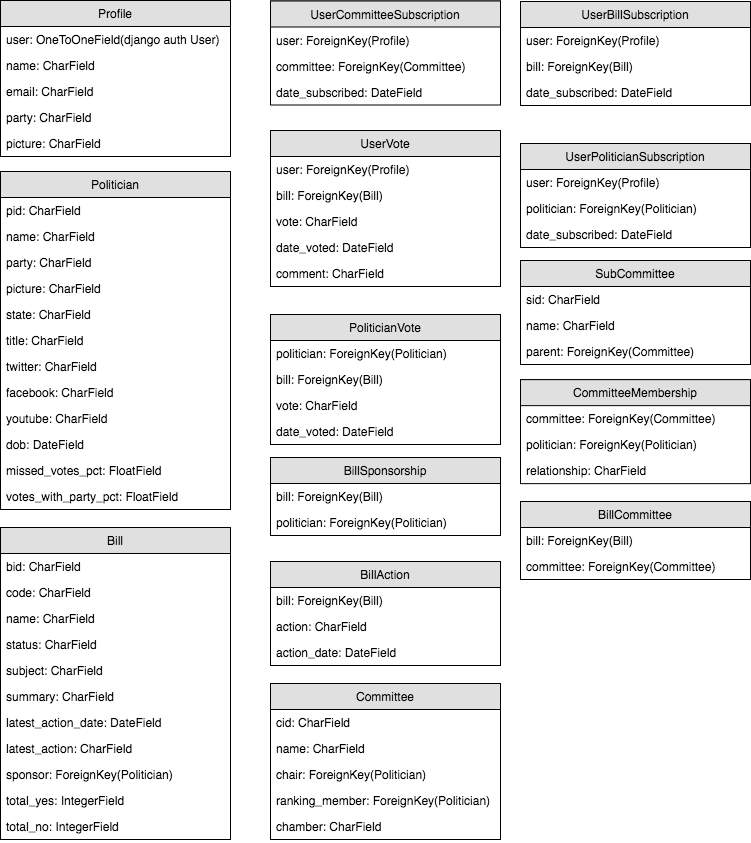
\includegraphics[scale=0.5]{politifind-data-model-UPDATED.png} \\

\n\textbf{URL Routes/Mappings}: 
\begin{center}
\begin{tabular}{ l | l | l }
route & name & description \\
\hline
r`\^{}\$' & index & route users to the home page \\
r`\^{}bill/(.*)/\$' & bill & individual bill page\\
r`\^{}politician/(.*)/(bills$\mid$votes)*' & politician & individual politician page\\
r`\^{}politicians/\$' & politicians & list of all politicians\\
r`\^{}bills/\$' & bills & list of all bills\\
r`\^{}committee/(.*)/(bills$\mid$subcomittees)*\$' & committee & individual committee page\\
r`\^{}committees/\$' & committees & list of all committees\\
r`\^{}profile/\$' & profile & user's profile page\\
r`\^{}search/\$' & search & display's search results\\
r`\^{}accounts/' & accounts & adds login/logout/etc urls\\
r`\^{}vote/(.*)/(yay$\mid$nay)*/' & vote & view individual vote page\\
r`\^{}subscribe/\$' & subscribe & user can subscribe\\
r`\^{}unsubscribe/\$' & unsubscribe & user can unsubscribe\\
r`\^{}profile/update/' & update profile & have a user update their profile page\\
\end{tabular}
\end{center}

\n\textbf{Authentication/Authorization}: We added a one-to-one mapping between Django's User model and our custom Profile model, allowing a user to specify additional information, such as political party, profile picture, etc.. Our users can browse Politifind without logging in, but when they do they have some additional functionality, such as subscribing to various politicians, bills, and committees, or voting on bills to see how they stack up against all politfind users and/or congress. We also enable to profile view to a logged in user where they can view all of their subscriptions and change their profile info. Lastly, the homepage is templated differently based on whether or not a user is logged in. We have one permissions group for a user that allows them to modify their info, or add votes and subscriptions, but it does not allow them to for example change the data of a bill, as it shouldn't. \\

\n\textbf{Team Choice}: For our team choice, we decided to integrate the Algolia Search API into our app to allow the user to very quickly search through all the data in politifind. To do this, we added two features. The first is an autocomplete search that reacts to what the user types in the search bar and displays results in a dropdown. this searching can happen from any of our views. The other feature is an actual search page. If a user does not want to look at the dropdown results, they can hit enter and it will bring them to a search page displaying the results from their query. We used the Algolia Javascript client for the autocompleting, and the algoliasearch-django pip module mentioned before for the search page. \\

\n\textbf{Conclusion}: \\

\end{document}
